%%%%%%%%%%%%%%%%%%%%%%%%%%%%%%%%%%%%%%%%%%%%
%%%%%%%%%%%%%%%%%%%%%%%%%%%%%%%%%%%%%%%%%%%%
% Import preamble
\input{../preamble_slides.tex}
\input{../abbreviations.tex}
%%%%%%%%%%%%%%%%%%%%%%%%%%%%%%%%%%%%%%%%%%%%
%%%%%%%%%%%%%%%%%%%%%%%%%%%%%%%%%%%%%%%%%%%%
% Define title


%\title{Climate survey - France}
%\author[OECD]{ \\  Antoine Dechezleprêtre, Adrien Fabre, Bluebery Planterose, Stefanie Stantcheva \\ (OECD) }
%
%              \date{}
              
\begin{document}



%%%%%%%%%%%%%%%%%%%%%%%%%%%%%%%%%%%%%%%%%%%%
%%%%%%%%%%%%%%%%%%%%%%%%%%%%%%%%%%%%%%%%%%%%
% Begin of the document
% TITLE PAGE

\begin{frame}
\thispagestyle{empty}
\begin{center}
\begin{LARGE}
\textcolor{blue}{Heterogenous Treatment Effects \& Policy Views Decomposition}
\end{LARGE}

\vspace{1cm}

Countries: US, France, Denmark, Germany
% Laurence Boone, Antoine Dechezleprêtre, Adrien Fabre, Tobias Kruse, Bluebery Planterose, Ana Sanchez-Chico, Stefanie Stantcheva \\

%\vspace{-0.3cm}

\DTMlangsetup{showdayofmonth=false}
\textit{\today} 

\end{center}

\bigskip

\end{frame}

\section{Heterogenous Treatment Effects}

\begin{frame}{Main Results}
\begin{itemize}
	\item Negative effect of Climate Treatment on right-wing respondents for support on policies, but policy treatment has positive effect on willingness to adopt climate friendly behavior.
	\item Both treatment have a negative effect on left-leaning people.
	\item Policy treatment has a negative effect on both right- and left-leaning people on thinking that rich people are responsible for CC \newline % TODO: specify that this is contrary to Center people. Specify what parties are considered Center, maybe present descriptive stats on left-right leaning before.
	\item Climate treatment has strong effects on the main origin/race of the country. \newline
	\item Also strong effects of both treatments on retired people and older people.
\end{itemize}
\end{frame}


\begin{frame}{}%\addtocounter{framenumber}{-1}
\begin{table}[h!]
%\caption{Heterogenous Treatment Effects -- Political}
\begin{center}
\scalebox{.46}{\input{../../tables/heterogeneity/main_results_het_left_right_all_small.tex}}
\end{center}
	{\fontsize{4}{6}\selectfont Note: Controls include categorical variables for having dominant origin in the country, gender, having children, college education,
income quartiles, employment tatus, age, political affiliation, living in an urban area, and the respondent's country.}
\end{table}
\end{frame}

\begin{frame}{}%\addtocounter{framenumber}{-1}
\begin{table}[h!]
\caption{Heterogenous Treatment Effects -- Origin}
\begin{center}
\scalebox{.44}{
\begin{tabular}{@{\extracolsep{5pt}}lcccccccc} 
\\[-1.8ex]\hline 
\hline \\[-1.8ex] 
\\[-1.8ex] & Knowledge Index & Index main policies & Index all policies & Index willing to change & Index global policies & Trust government & Companies Responsible & Rich responsible \\ 
\hline \\[-1.8ex] 
 Control group mean & 0 & -0.106 & -0.067 & 0.002 & -0.028 & 0.27 & 0.721 & 0.433  \\ \hline \\[-1.8ex] origin: largest group & 0.043$^{*}$ & $-$0.201$^{***}$ & $-$0.151$^{***}$ & $-$0.094 & $-$0.168$^{***}$ & $-$0.034 & $-$0.038 & $-$0.016 \\ 
  & (0.026) & (0.057) & (0.057) & (0.058) & (0.058) & (0.027) & (0.026) & (0.030) \\ 
 origin: largest group $\times$ Treatment Climate & 0.002 & 0.260$^{***}$ & 0.197$^{**}$ & 0.289$^{***}$ & 0.152$^{*}$ & 0.030 & 0.071$^{*}$ & 0.005 \\ 
  & (0.038) & (0.085) & (0.085) & (0.087) & (0.086) & (0.040) & (0.039) & (0.044) \\ 
 origin: largest group $\times$ Treatment Policy & $-$0.019 & 0.124 & 0.093 & 0.105 & 0.109 & 0.024 & 0.030 & 0.044 \\ 
  & (0.038) & (0.084) & (0.084) & (0.086) & (0.085) & (0.039) & (0.038) & (0.043) \\ 
 origin: largest group $\times$ Treatment Both & 0.038 & 0.336$^{***}$ & 0.271$^{***}$ & 0.297$^{***}$ & 0.220$^{**}$ & 0.018 & 0.104$^{***}$ & 0.076$^{*}$ \\ 
  & (0.039) & (0.085) & (0.085) & (0.087) & (0.087) & (0.040) & (0.039) & (0.044) \\ 
\hline \\[-1.8ex] 

Observations & 8,010 & 8,010 & 8,010 & 8,010 & 8,010 & 8,010 & 8,010 & 8,010 \\ 
\hline 
\hline \\[-1.8ex] 
\end{tabular} }
\end{center}
\end{table}
\end{frame}

\begin{frame}{}%\addtocounter{framenumber}{-1}
\begin{table}[h!]
%\caption{Heterogenous Treatment Effects -- Employment}
\begin{center}
\scalebox{.46}{
\begin{tabular}{@{\extracolsep{5pt}}lcccccccc} 
\\[-1.8ex]\hline 
\hline \\[-1.8ex] 
\\[-1.8ex] & Knowledge Index & Index main policies & Index all policies & Index willing to change & Index global policies & Trust government & Companies Responsible & Rich responsible \\ 
\hline \\[-1.8ex] 
 Control group mean & 0 & -0.103 & -0.055 & 0.002 & -0.028 & 0.27 & 0.721 & 0.433  \\ \hline \\[-1.8ex] Retired & $-$0.020 & $-$0.039 & $-$0.060 & $-$0.079 & $-$0.083 & 0.025 & $-$0.016 & 0.031 \\ 
  & (0.033) & (0.073) & (0.073) & (0.075) & (0.075) & (0.034) & (0.034) & (0.038) \\ 
 Student & 0.158$^{***}$ & 0.080 & 0.090 & 0.023 & 0.074 & 0.056 & 0.081$^{*}$ & $-$0.032 \\ 
  & (0.046) & (0.102) & (0.101) & (0.104) & (0.104) & (0.047) & (0.047) & (0.053) \\ 
 Working & 0.021 & 0.023 & 0.023 & $-$0.066 & 0.030 & 0.071$^{**}$ & $-$0.012 & $-$0.061$^{*}$ \\ 
  & (0.029) & (0.065) & (0.065) & (0.066) & (0.066) & (0.030) & (0.030) & (0.034) \\ 
  & (0.039) & (0.087) & (0.087) & (0.089) & (0.088) & (0.040) & (0.040) & (0.045) \\ 
 Retired $\times$ Treatment Climate & 0.032 & 0.087 & 0.186$^{*}$ & 0.104 & 0.237$^{**}$ & 0.033 & 0.022 & $-$0.082 \\ 
  & (0.046) & (0.102) & (0.101) & (0.104) & (0.104) & (0.047) & (0.046) & (0.053) \\ 
 Student $\times$ Treatment Climate & $-$0.047 & $-$0.034 & 0.053 & 0.054 & 0.173 & 0.051 & $-$0.019 & $-$0.033 \\ 
  & (0.069) & (0.152) & (0.152) & (0.155) & (0.155) & (0.071) & (0.070) & (0.079) \\ 
 Working $\times$ Treatment Climate & $-$0.007 & 0.019 & 0.081 & 0.092 & 0.121 & 0.005 & 0.021 & 0.013 \\ 
  & (0.043) & (0.096) & (0.096) & (0.098) & (0.098) & (0.045) & (0.044) & (0.050) \\ 
 Retired $\times$ Treatment Policy & 0.039 & 0.144 & 0.083 & 0.048 & 0.098 & 0.009 & $-$0.045 & $-$0.090$^{*}$ \\ 
  & (0.046) & (0.102) & (0.102) & (0.104) & (0.104) & (0.048) & (0.047) & (0.053) \\ 
 Student $\times$ Treatment Policy & $-$0.058 & $-$0.072 & $-$0.050 & $-$0.110 & $-$0.031 & 0.085 & $-$0.140$^{**}$ & $-$0.113 \\ 
  & (0.065) & (0.143) & (0.143) & (0.146) & (0.145) & (0.067) & (0.065) & (0.074) \\ 
 Working $\times$ Treatment Policy & 0.025 & 0.021 & $-$0.053 & 0.021 & $-$0.018 & $-$0.054 & $-$0.098$^{**}$ & $-$0.036 \\ 
  & (0.043) & (0.096) & (0.096) & (0.098) & (0.098) & (0.045) & (0.044) & (0.050) \\ 
 Retired $\times$ Treatment Both & $-$0.026 & 0.323$^{***}$ & 0.301$^{***}$ & 0.360$^{***}$ & 0.209$^{**}$ & $-$0.011 & 0.076 & 0.023 \\ 
  & (0.047) & (0.103) & (0.103) & (0.106) & (0.105) & (0.048) & (0.047) & (0.053) \\ 
 Student $\times$ Treatment Both & $-$0.075 & 0.125 & 0.177 & 0.044 & 0.016 & 0.006 & $-$0.044 & $-$0.092 \\ 
  & (0.067) & (0.148) & (0.148) & (0.151) & (0.151) & (0.069) & (0.068) & (0.077) \\ 
 Working $\times$ Treatment Both & $-$0.070 & 0.140 & 0.170$^{*}$ & 0.237$^{**}$ & 0.089 & $-$0.011 & 0.060 & 0.079 \\ 
  & (0.043) & (0.096) & (0.096) & (0.098) & (0.097) & (0.045) & (0.044) & (0.049) \\ 
\hline \\[-1.8ex] 

Observations & 8,010 & 8,010 & 8,010 & 8,010 & 8,010 & 8,010 & 8,010 & 8,010 \\ 
\hline 
\hline \\[-1.8ex] 
\end{tabular} }
\end{center}
\end{table}
\end{frame}

\begin{frame}{}%\addtocounter{framenumber}{-1}
\begin{table}[h!]
%\caption{Heterogenous Treatment Effects -- Age}
\begin{center}
\scalebox{.45}{
\begin{tabular}{@{\extracolsep{5pt}}lcccccccc} 
\\[-1.8ex]\hline 
\hline \\[-1.8ex] 
\\[-1.8ex] & Knowledge Index & Index main policies & Index all policies & Index willing to change & Index global policies & Trust government & Companies Responsible & Rich responsible \\ 
\hline \\[-1.8ex] 
 Age: 25-34 & $-$0.063$^{*}$ & $-$0.026 & 0.064 & $-$0.023 & 0.163$^{**}$ & 0.028 & 0.014 & $-$0.036 \\ 
  & (0.036) & (0.080) & (0.080) & (0.082) & (0.081) & (0.037) & (0.037) & (0.041) \\ 
 Age: 35-49 & $-$0.040 & $-$0.116 & 0.007 & $-$0.217$^{***}$ & 0.053 & 0.029 & $-$0.024 & $-$0.027 \\ 
  & (0.035) & (0.077) & (0.077) & (0.079) & (0.078) & (0.036) & (0.035) & (0.040) \\ 
 Age: 50-64 & 0.030 & $-$0.125 & $-$0.025 & $-$0.209$^{***}$ & $-$0.010 & 0.032 & 0.007 & $-$0.068$^{*}$ \\ 
  & (0.034) & (0.076) & (0.076) & (0.078) & (0.078) & (0.036) & (0.035) & (0.039) \\ 
 Age: 65+ & 0.056 & $-$0.269$^{***}$ & $-$0.106 & $-$0.446$^{***}$ & $-$0.040 & 0.030 & $-$0.019 & $-$0.066 \\ 
  & (0.037) & (0.082) & (0.082) & (0.084) & (0.083) & (0.038) & (0.037) & (0.042) \\ 
 Age: 25-34 $\times$ Treatment Climate & $-$0.039 & $-$0.136 & $-$0.207$^{*}$ & $-$0.035 & $-$0.350$^{***}$ & 0.003 & $-$0.031 & $-$0.027 \\ 
  & (0.053) & (0.118) & (0.118) & (0.121) & (0.120) & (0.055) & (0.054) & (0.061) \\ 
 Age: 35-49 $\times$ Treatment Climate & $-$0.021 & $-$0.064 & $-$0.140 & 0.096 & $-$0.178 & 0.010 & 0.032 & $-$0.002 \\ 
  & (0.050) & (0.110) & (0.110) & (0.112) & (0.112) & (0.051) & (0.050) & (0.057) \\ 
 Age: 50-64 $\times$ Treatment Climate & $-$0.028 & $-$0.222$^{**}$ & $-$0.254$^{**}$ & $-$0.067 & $-$0.206$^{*}$ & $-$0.012 & 0.006 & $-$0.059 \\ 
  & (0.049) & (0.109) & (0.108) & (0.111) & (0.111) & (0.051) & (0.050) & (0.056) \\ 
 Age: 65+ $\times$ Treatment Climate & 0.019 & $-$0.020 & $-$0.072 & 0.099 & $-$0.128 & 0.031 & 0.001 & $-$0.107$^{*}$ \\ 
  & (0.049) & (0.108) & (0.108) & (0.111) & (0.110) & (0.051) & (0.050) & (0.056) \\ 
 Age: 25-34 $\times$ Treatment Policy & 0.100$^{*}$ & $-$0.051 & $-$0.089 & $-$0.031 & $-$0.171 & $-$0.048 & 0.069 & 0.006 \\ 
  & (0.051) & (0.113) & (0.112) & (0.115) & (0.115) & (0.053) & (0.052) & (0.058) \\ 
 Age: 35-49 $\times$ Treatment Policy & 0.110$^{**}$ & 0.075 & $-$0.023 & 0.097 & $-$0.042 & $-$0.077 & 0.069 & $-$0.063 \\ 
  & (0.048) & (0.107) & (0.107) & (0.109) & (0.109) & (0.050) & (0.049) & (0.055) \\ 
 Age: 50-64 $\times$ Treatment Policy & 0.053 & $-$0.014 & $-$0.093 & $-$0.096 & $-$0.065 & $-$0.107$^{**}$ & 0.017 & $-$0.046 \\ 
  & (0.047) & (0.104) & (0.104) & (0.107) & (0.106) & (0.049) & (0.048) & (0.054) \\ 
 Age: 65+ $\times$ Treatment Policy & 0.132$^{***}$ & 0.127 & 0.074 & 0.080 & 0.070 & $-$0.088$^{*}$ & 0.078$^{*}$ & $-$0.068 \\ 
  & (0.047) & (0.104) & (0.104) & (0.106) & (0.106) & (0.048) & (0.048) & (0.054) \\ 
 Age: 25-34 $\times$ Treatment Both & 0.039 & $-$0.070 & $-$0.093 & $-$0.019 & $-$0.185 & $-$0.018 & 0.024 & 0.089 \\ 
  & (0.052) & (0.115) & (0.115) & (0.117) & (0.117) & (0.054) & (0.053) & (0.059) \\ 
 Age: 35-49 $\times$ Treatment Both & $-$0.023 & $-$0.002 & $-$0.010 & 0.075 & 0.022 & 0.017 & 0.103$^{**}$ & 0.078 \\ 
  & (0.049) & (0.108) & (0.107) & (0.110) & (0.110) & (0.050) & (0.049) & (0.056) \\ 
 Age: 50-64 $\times$ Treatment Both & 0.052 & 0.039 & 0.026 & 0.057 & 0.120 & 0.008 & 0.052 & 0.086 \\ 
  & (0.048) & (0.106) & (0.106) & (0.109) & (0.108) & (0.050) & (0.049) & (0.055) \\ 
 Age: 65+ $\times$ Treatment Both & 0.096$^{**}$ & 0.270$^{**}$ & 0.203$^{*}$ & 0.298$^{***}$ & 0.199$^{*}$ & $-$0.030 & 0.113$^{**}$ & 0.074 \\ 
  & (0.049) & (0.108) & (0.108) & (0.111) & (0.110) & (0.051) & (0.050) & (0.056) \\ 
\hline \\[-1.8ex] 

Observations & 8,010 & 8,010 & 8,010 & 8,010 & 8,010 & 8,010 & 8,010 & 8,010 \\ 
\hline 
\hline \\[-1.8ex] 
\end{tabular} }
\end{center}
\end{table}
\end{frame}

\section{Decomposition of Policy Views}


\begin{frame}{Main Results}
\begin{itemize}
	\item Political leaning and age are important drivers of support. \newline
	\item Belief in efficiency and fairness are key.
	\item Thinking that climate change will/is affect(ing) oneself is much more important than being actually vulnerable to climate change. \newline
	\item Partisan gap is also explained by different views on the efficiency of climate policies, as well as the importance of addressing poverty and inequalities, and not so much by objective characteristics (e.g., being vulnerable to CC or financially constrained).
	\item The geographical gap is largely explained by feeling affected by CC.
	\item Being concerned about climate change only plays a secondary role. \newline
	\item Support is largely idiosyncratic: political leaning explains 8\% of the variance, socio-demographics less than 2\%
\end{itemize}
\end{frame}


\begin{frame}{Variance Decomposition of Policy Support -- Individual Characteristics}%\addtocounter{framenumber}{-1}
\vspace{-.1cm}
{\footnotesize $R^2$ = 10\%}
\begin{figure}[h!]
\vspace{-.1cm}
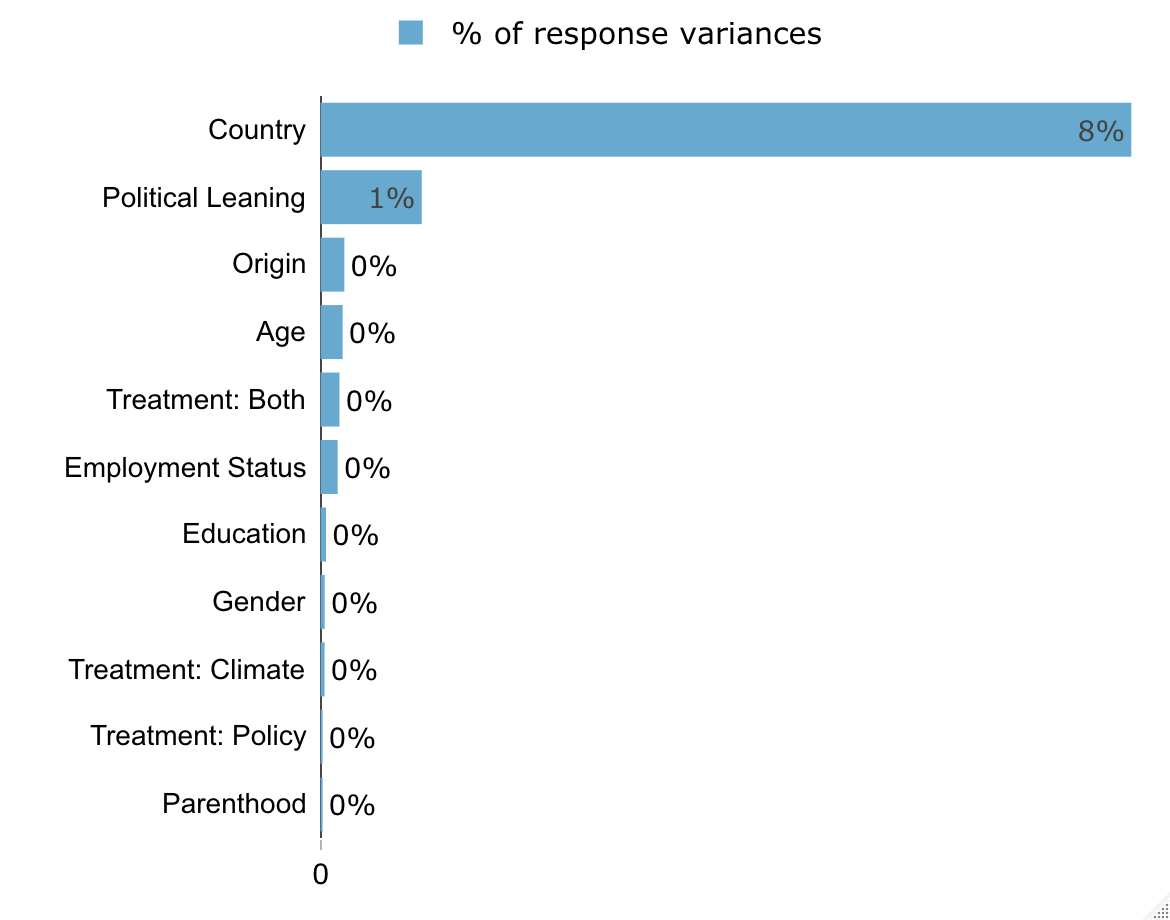
\includegraphics[width=.64\textwidth]{../../figures/Gelbach/lmg_all_policies_no_indices_non_standardized} \\
%\caption{Could you trust the federal goverment to implement the following policies}
\end{figure}
\end{frame}

\begin{frame}{Variance Decomposition of Policy Support -- Individual Characteristics and Indices}%\addtocounter{framenumber}{-1}
\vspace{-.1cm}
{\footnotesize $R^2$ = 68\%}
\begin{figure}[h!]
\vspace{-.15cm}
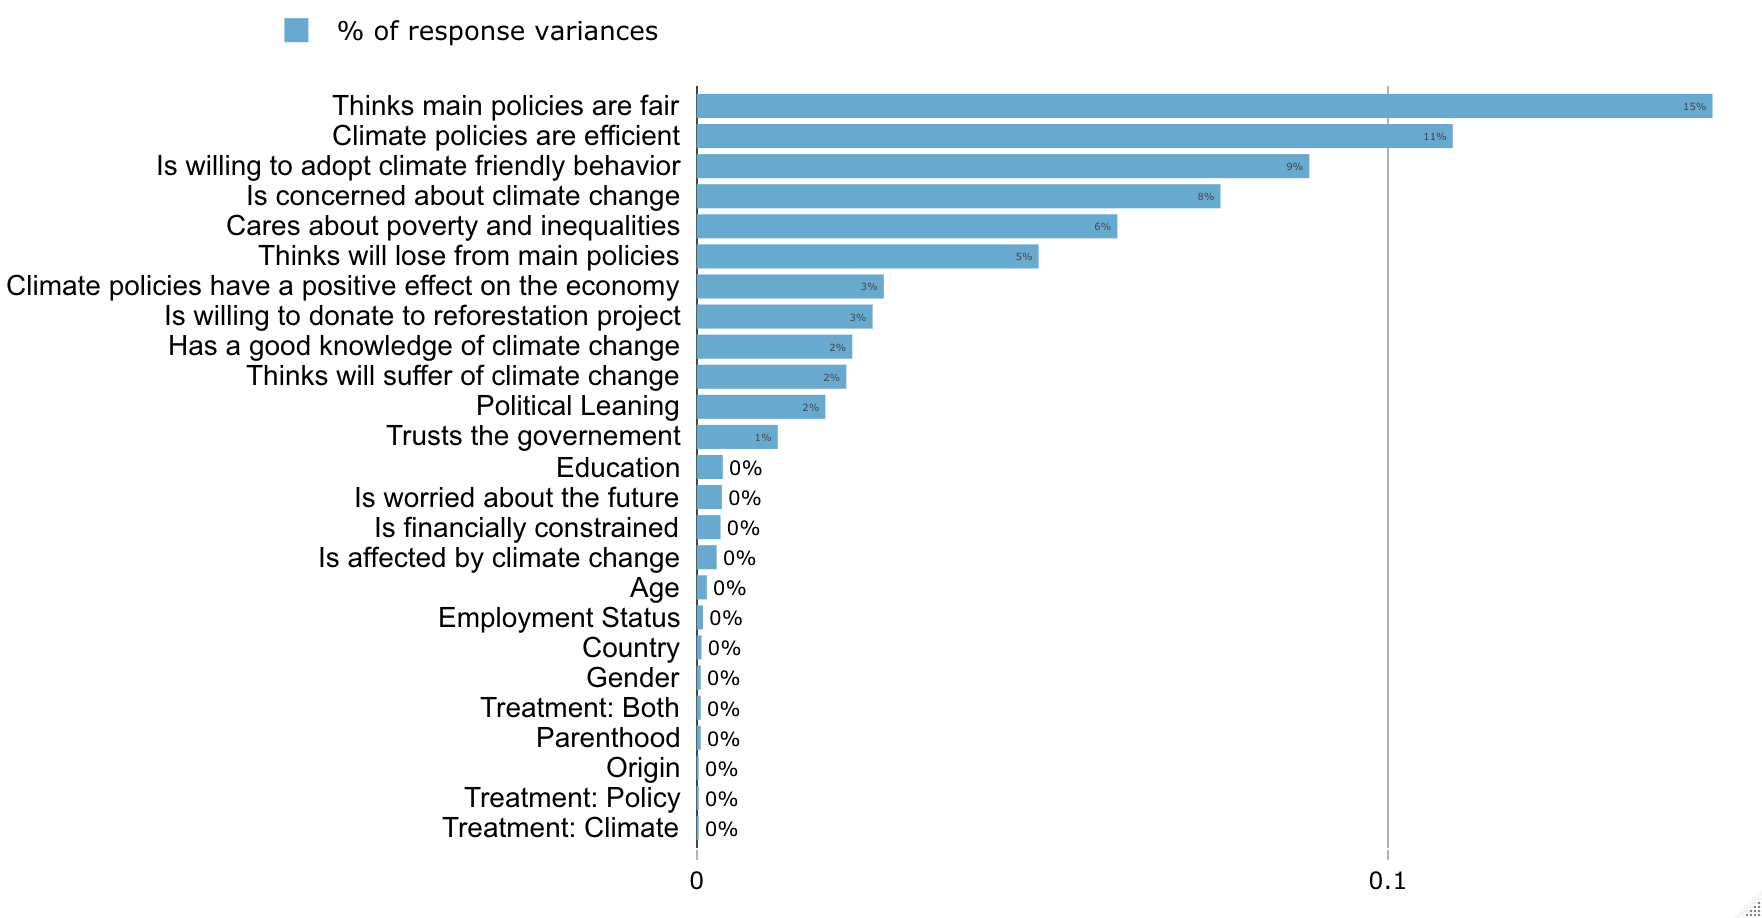
\includegraphics[width=1\textwidth]{../../figures/Gelbach/lmg_all_policies_w_controls_non_standardized} \\
%\caption{Could you trust the federal goverment to implement the following policies}
\end{figure}
\end{frame}

\begin{frame}{Variance Decomposition of Policy Support -- Indices}%\addtocounter{framenumber}{-1}
\vspace{-.1cm}
{\footnotesize $R^2$ = 68\% 22 regressors explaining 10\% of the variance are always included in the ANOVAs. The remaining variance (58\%) decomposes as follows:}
\begin{figure}[h!]
\vspace{-.2cm}
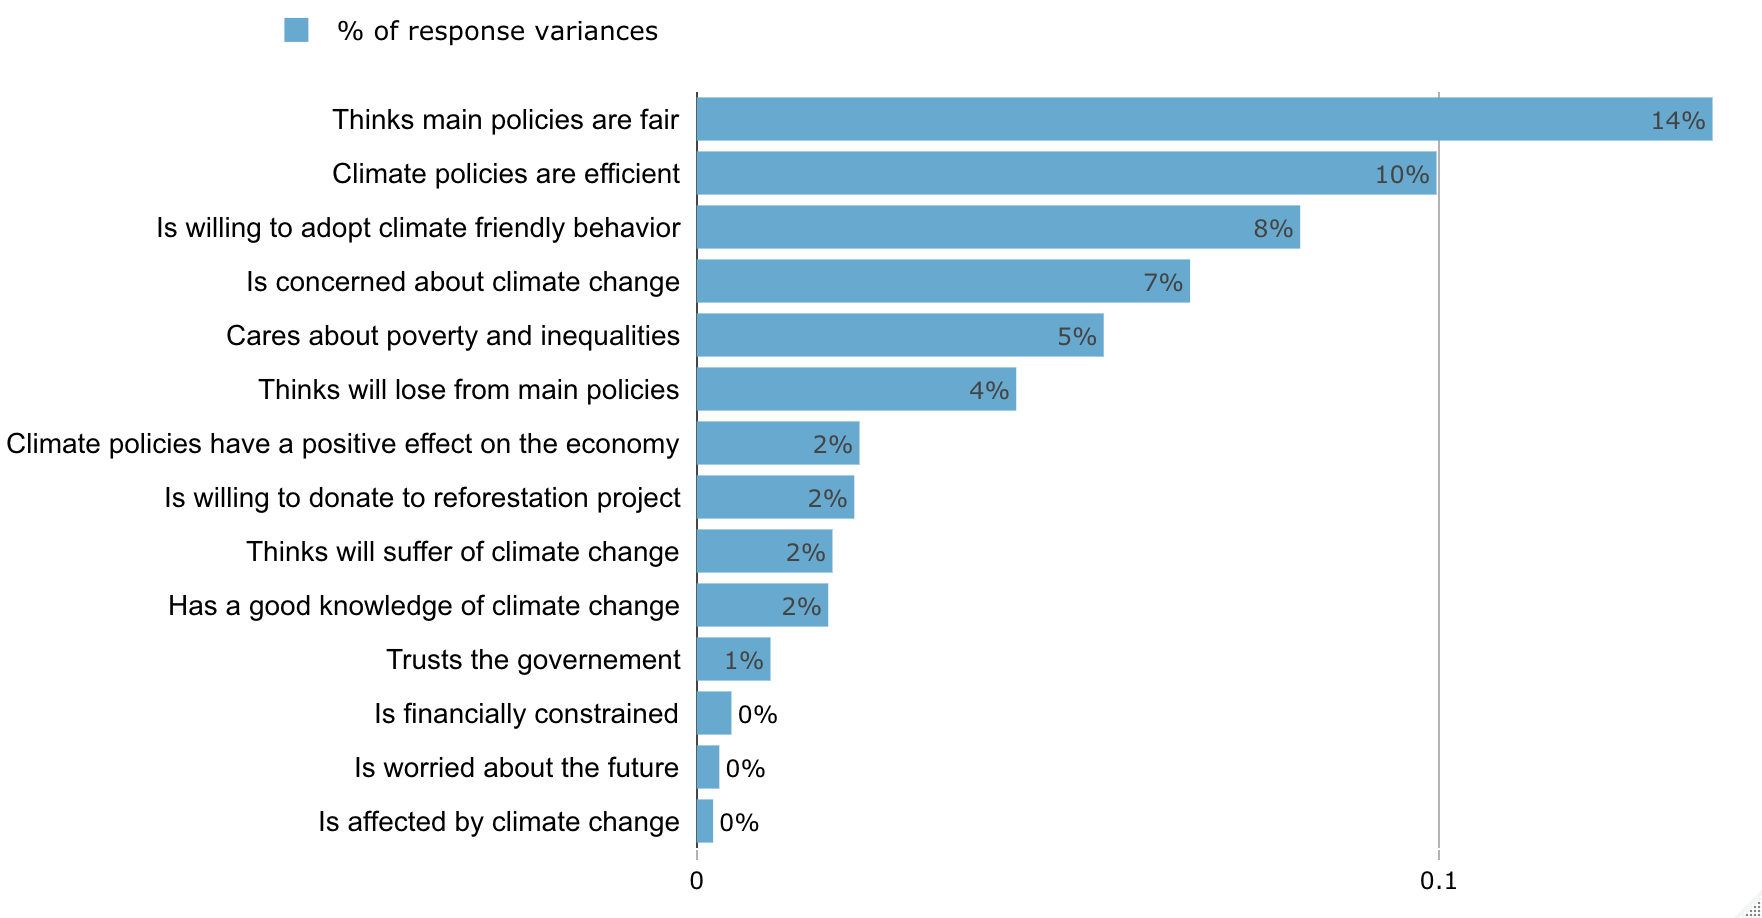
\includegraphics[width=.9\textwidth]{../../figures/Gelbach/lmg_all_policies_non_standardized} \\
%\caption{Could you trust the federal goverment to implement the following policies}
\end{figure}
\end{frame}


\begin{frame}{Variance Decomposition of Willingness to Adapt -- Individual Characteristics}%\addtocounter{framenumber}{-1}
\vspace{-.1cm}
{\footnotesize $R^2$ = 6\%}
\begin{figure}[h!]
\vspace{-.1cm}
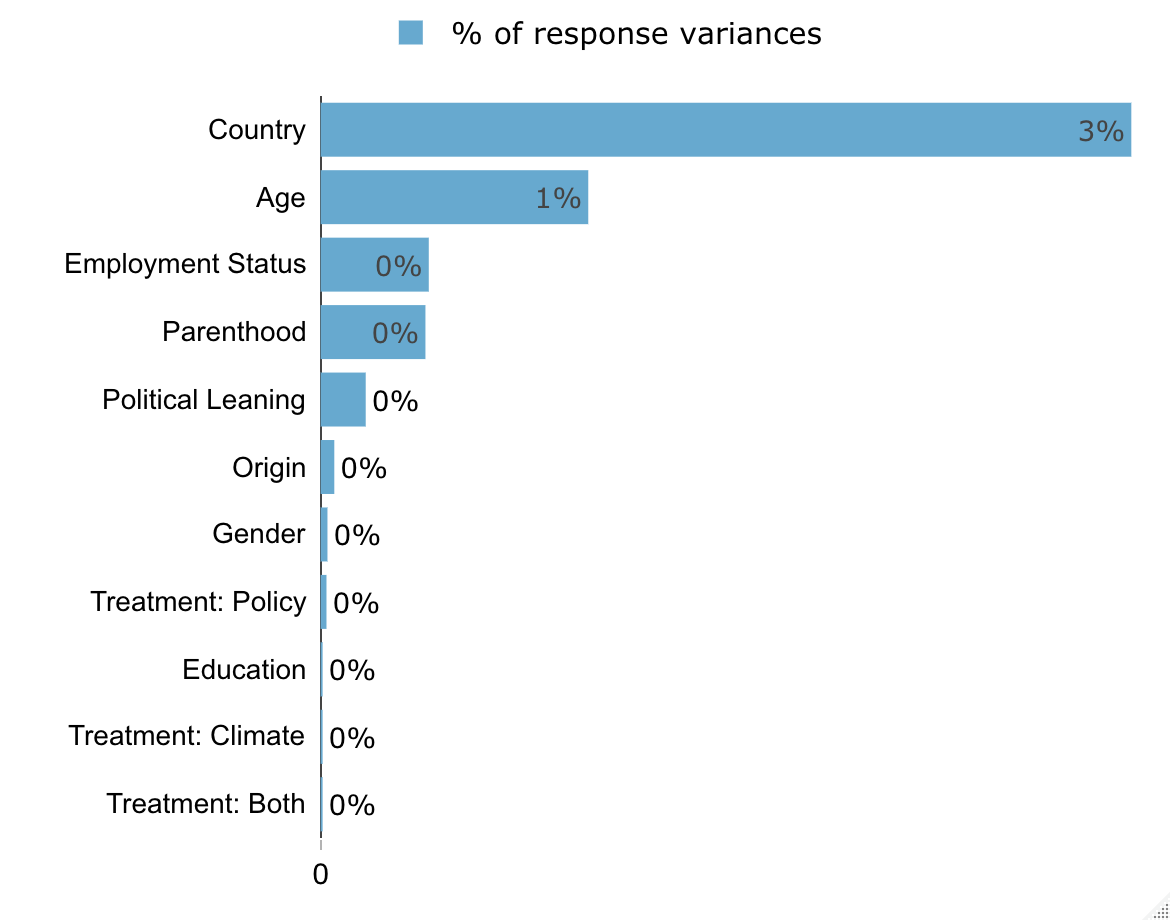
\includegraphics[width=.64\textwidth]{../../figures/Gelbach/lmg_willing_change_no_indices_non_standardized} \\
%\caption{Could you trust the federal goverment to implement the following policies}
\end{figure}
\end{frame}

\begin{frame}{Variance Decomposition of Willingness to Adapt -- Indiv. Characteristics and Indices}%\addtocounter{framenumber}{-1}
\vspace{-.15cm}
{\footnotesize $R^2$ = 39\%}
\begin{figure}[h!]
\vspace{-.15cm}
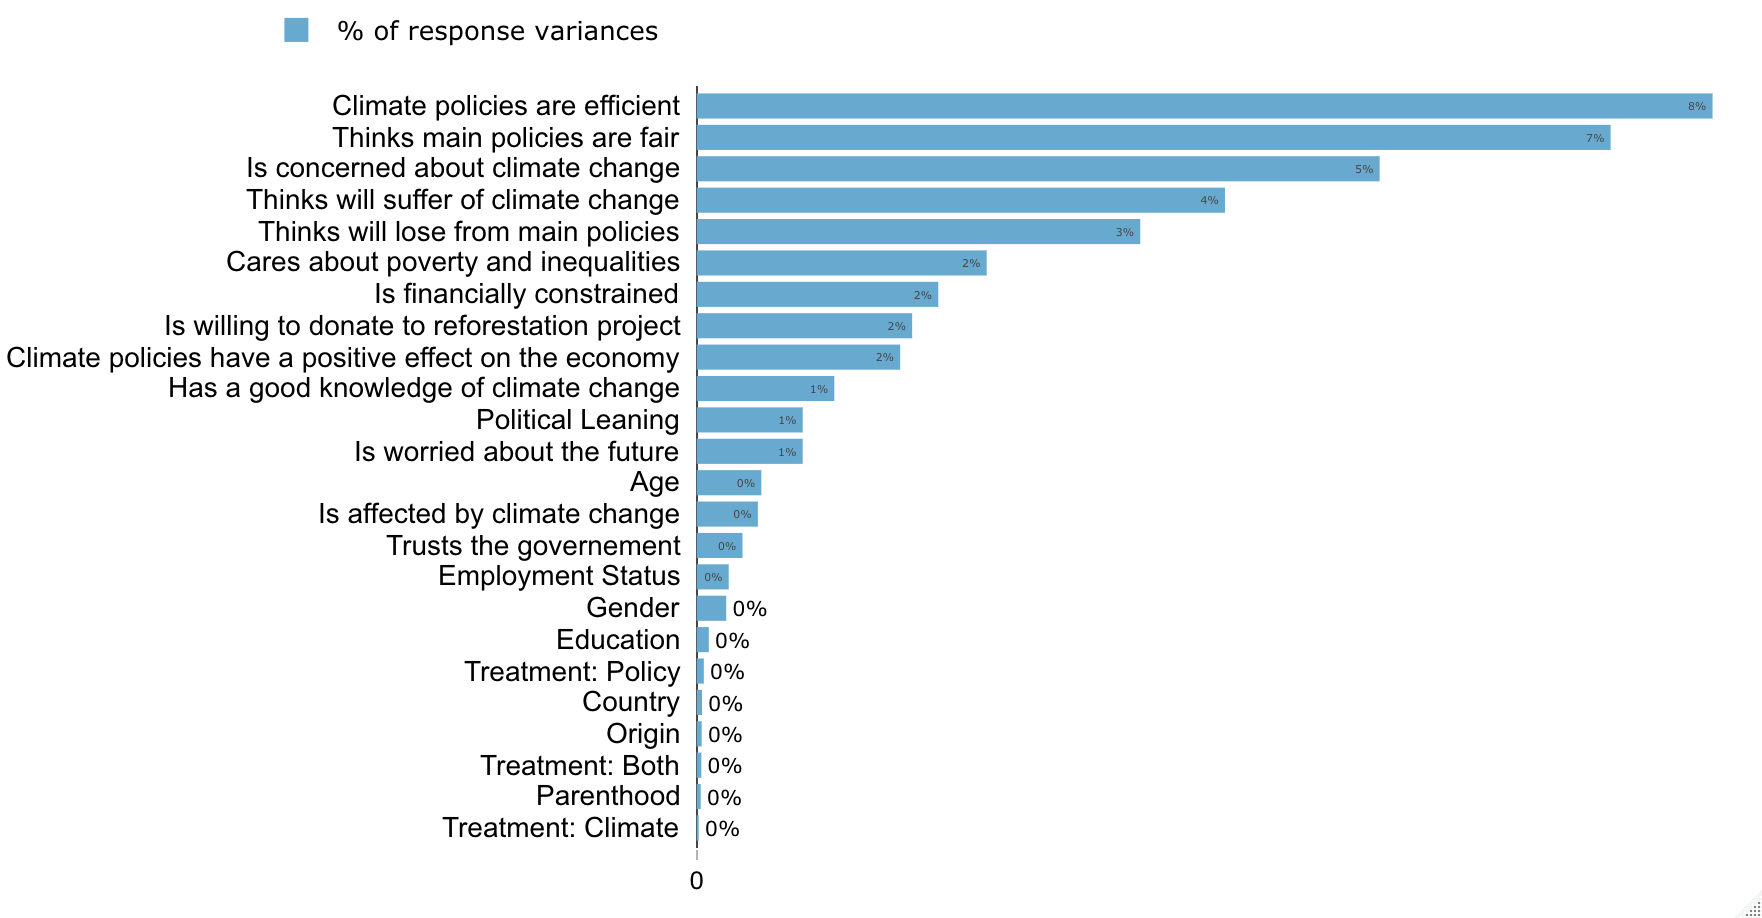
\includegraphics[width=1\textwidth]{../../figures/Gelbach/lmg_willing_change_w_controls_non_standardized} \\
%\caption{Could you trust the federal goverment to implement the following policies}
\end{figure}
\end{frame}

\begin{frame}{Variance Decomposition of Willingness to Adapt -- Indices}%\addtocounter{framenumber}{-1}
\vspace{-.1cm}
{\footnotesize $R^2$ = 39\% 22 regressors explaining 6\% of the variance are always included in the ANOVAs. The remaining variance (34\%) decomposes as follows:}
\begin{figure}[h!]
\vspace{-.1cm}
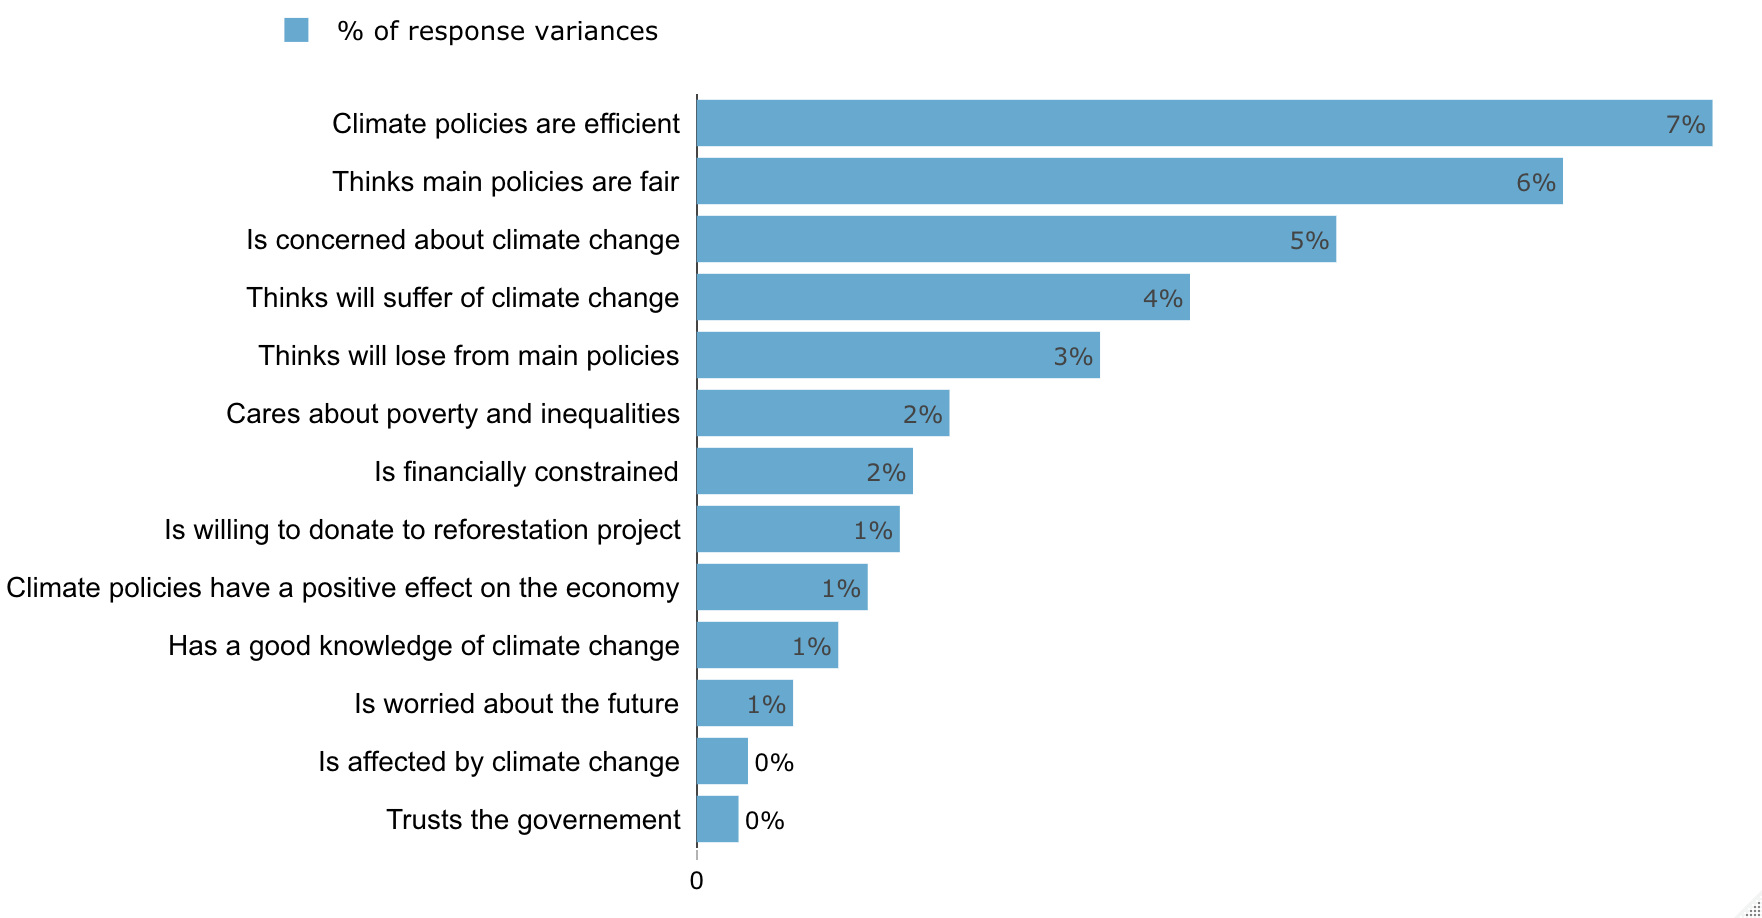
\includegraphics[width=.9\textwidth]{../../figures/Gelbach/lmg_willing_change_non_standardized} \\
%\caption{Could you trust the federal goverment to implement the following policies}
\end{figure}
\end{frame}



\begin{frame}{Decomposing Policy View -- Individual Characteristics}%\addtocounter{framenumber}{-1}
\begin{figure}[h!]
\includegraphics[width=.75\textwidth]{../../figures/Gelbach/coef_policy_views_all} \\
%\caption{Could you trust the federal goverment to implement the following policies}
{\tiny \textit{Notes:} In this figure, the dependent variable are policy indices. Depicted are coefficients on different types of variables and from two different specifications. We show the coefficients from the regressions of each policy index on (only) treatment indicators and on the full set of individual covariates.}
\end{figure}
\end{frame}

\begin{frame}{Decomposing Policy View -- Mechanisms}%\addtocounter{framenumber}{-1}
\begin{figure}[h!]
\includegraphics[width=.9\textwidth]{../../figures/Gelbach/coef_policy_views_indices_all} \\
%\caption{Could you trust the federal goverment to implement the following policies}
{\tiny \textit{Notes:} We show the coefficients on the different policy views from the regressions of each policy index on these factors, controlling for the full array of individual covariates and treatment indicators. We do not show the coefficients on all individual-level controls, except for the coefficient on the political indicators.}
\end{figure}
\end{frame}

\begin{frame}{Gelbach decomposition of the partisan gap in support for…}%\addtocounter{framenumber}{-1}
\vspace{-.2cm}
\begin{figure}[h!]
\caption{… all climate policies}
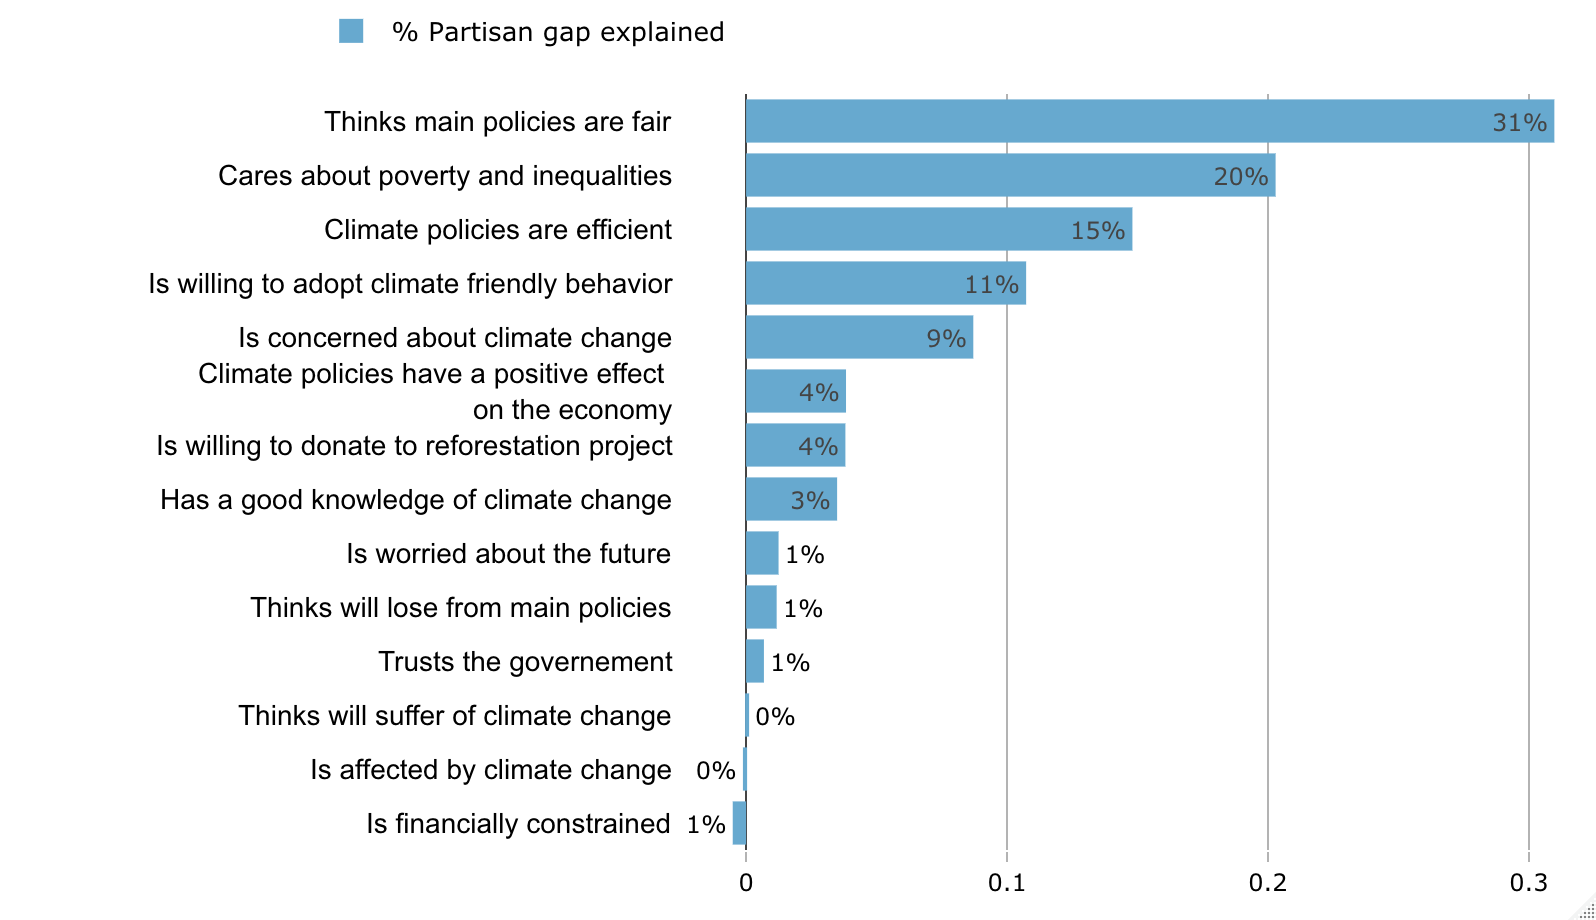
\includegraphics[width=.75\textwidth]{../../figures/Gelbach/gelbach_right_all_policies_D2SD} \\
%\caption{Could you trust the federal goverment to implement the following policies}
{\tiny \textit{Notes:} Each bar indicates the share of the partisan gap explained by each of the factors.}
\end{figure}
\end{frame}

\begin{frame}{Explaining the Partisan Gap}
\begin{figure}[h!]
	\caption{Gelbach decomposition of the partisan gap in support for:}
	\setlength\extrarowheight{-1pt}
\begin{center}
	\begin{tabular}{cc}
		\begin{subfigure}{0.48\textwidth}
		\caption{Ban on combustion-engine cars}
			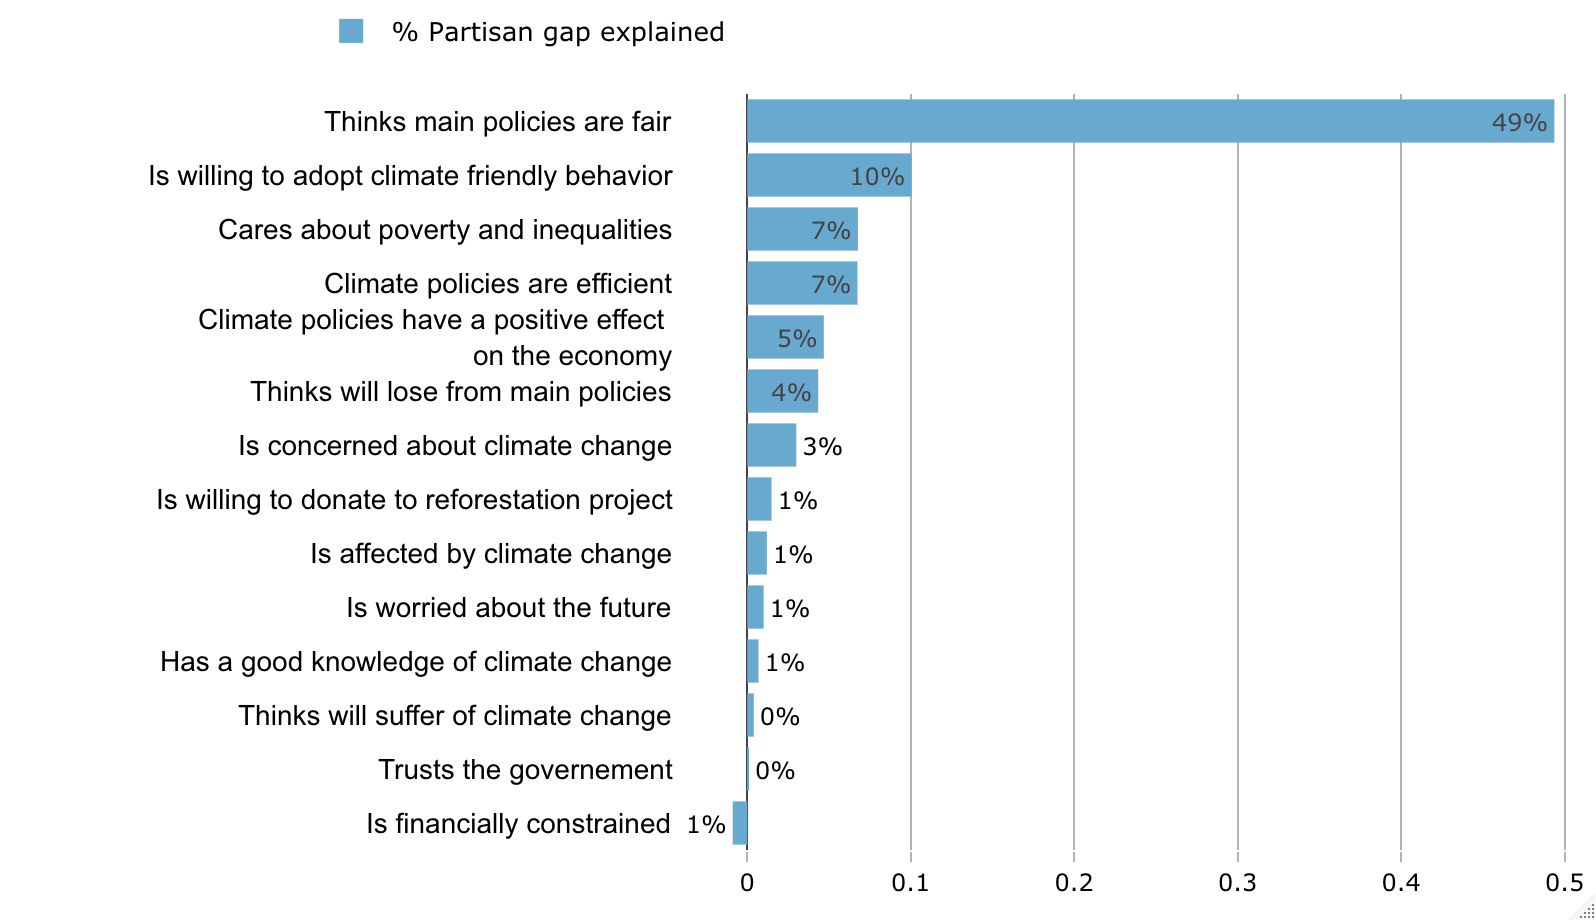
\includegraphics[width=\textwidth]{../../figures/Gelbach/gelbach_right_standard_D2SD}
		\end{subfigure}&
		\begin{subfigure}{0.48\textwidth}
		\caption{Carbon tax with cash transfers}
			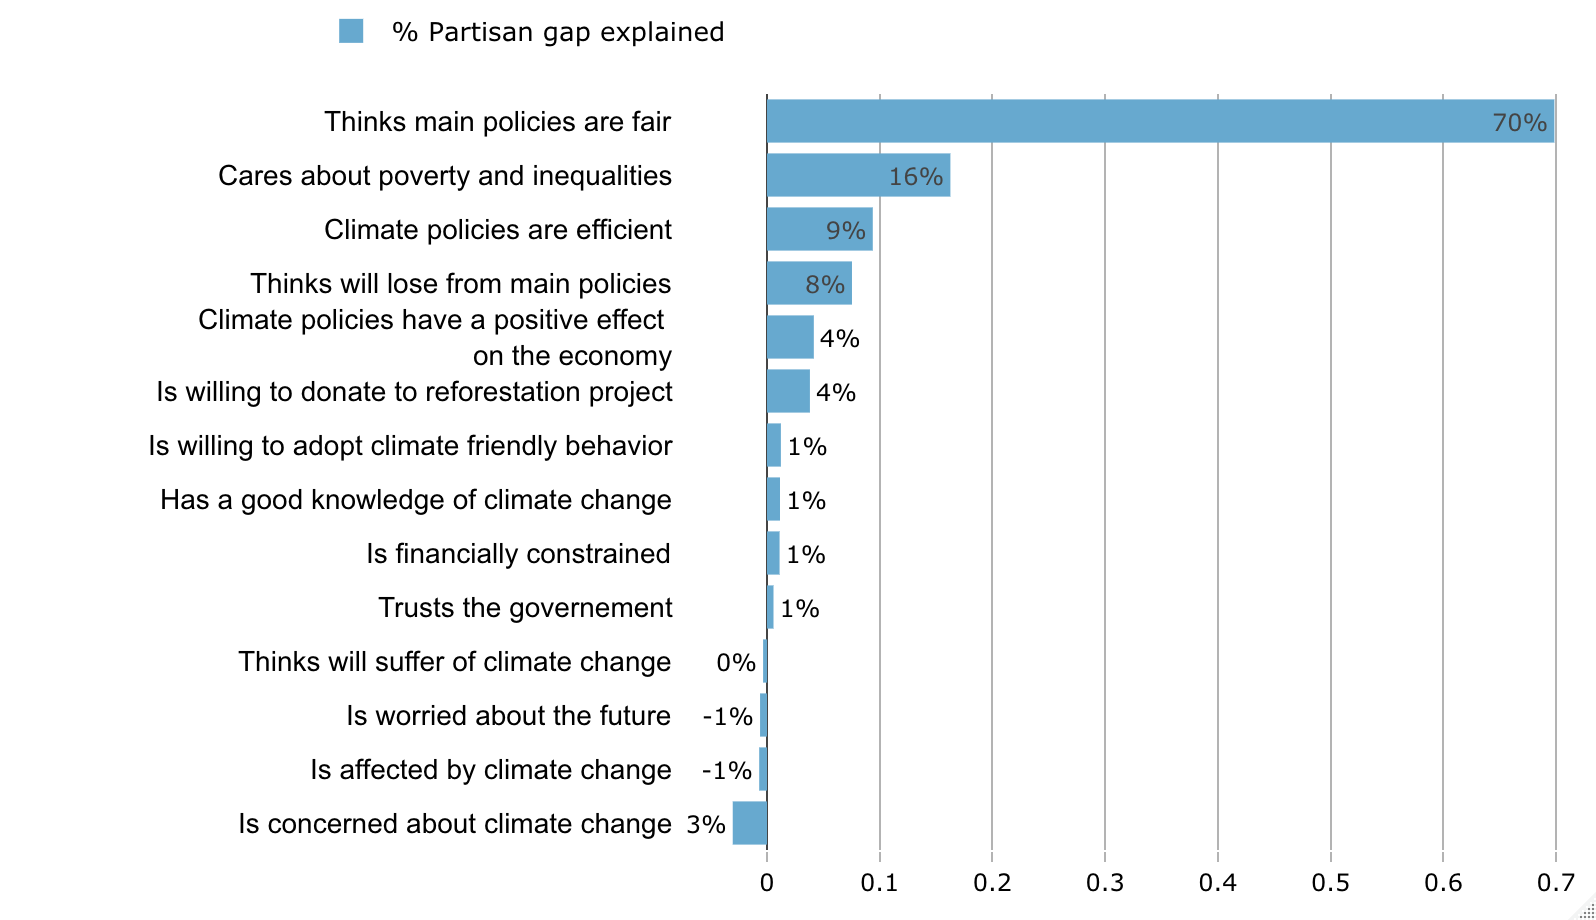
\includegraphics[width=\textwidth]{../../figures/Gelbach/gelbach_right_tax_transfers_D2SD}
		\end{subfigure}\\
	\end{tabular}
\end{center}
\end{figure}
\end{frame}

\begin{frame}{Explaining the Partisan Gap}
\begin{figure}[h!]
	\caption{Gelbach decomposition of the partisan gap in support for:}
	\setlength\extrarowheight{-1pt}
\begin{center}
	\begin{tabular}{cc}
		\begin{subfigure}{0.48\textwidth}
		\caption{Green investment program}
			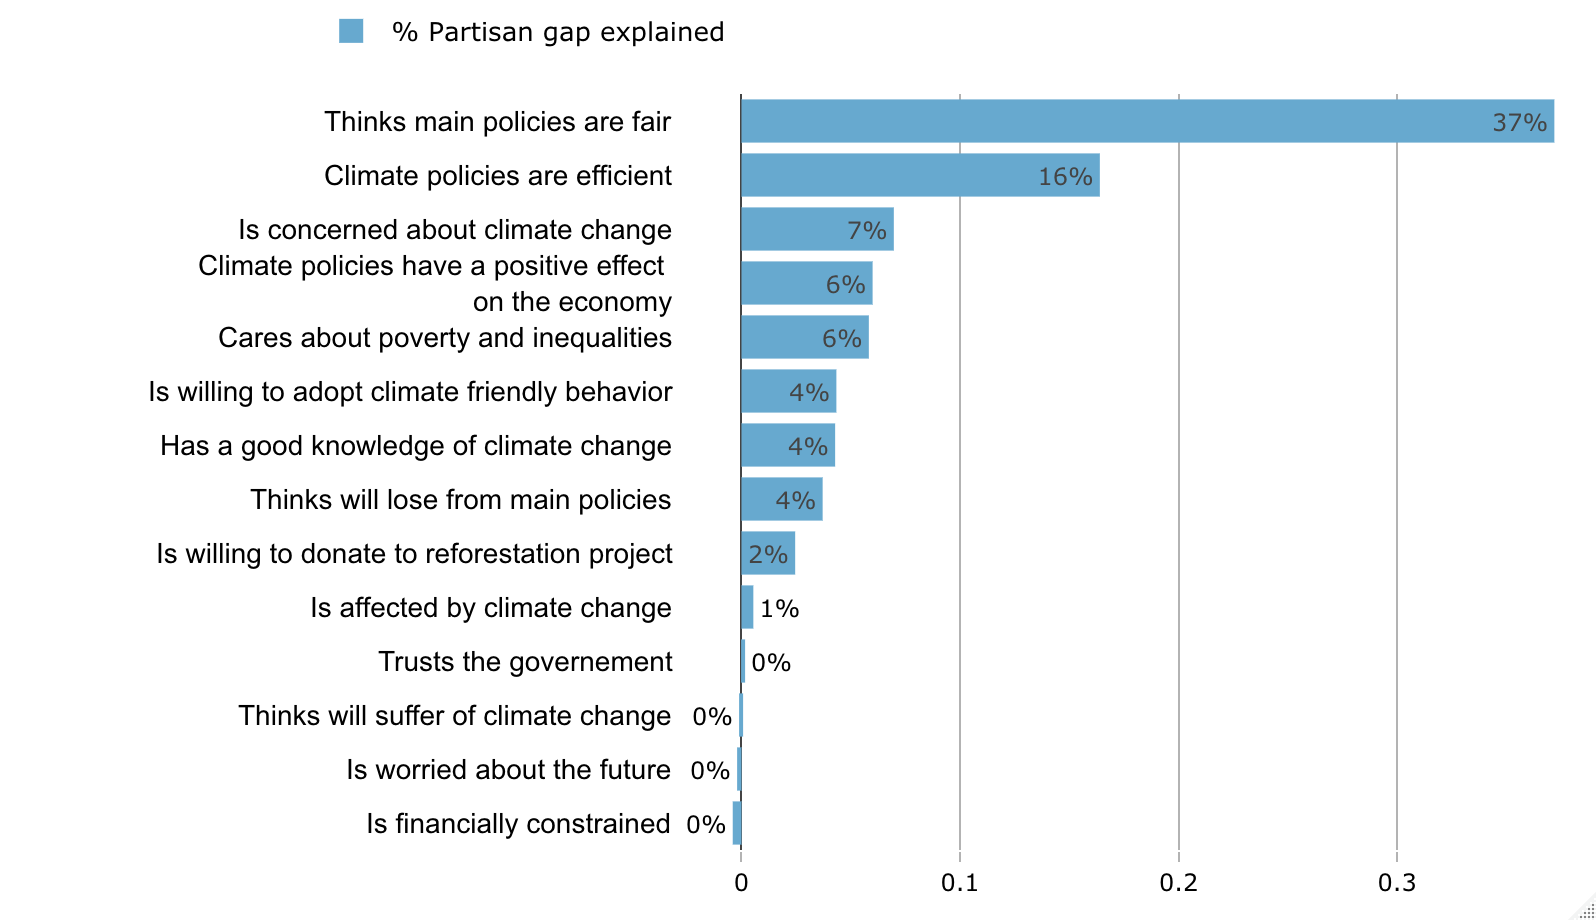
\includegraphics[width=\textwidth]{../../figures/Gelbach/gelbach_right_investments_D2SD}
		\end{subfigure}&
		\begin{subfigure}{0.48\textwidth}
		\caption{All 3 policies}
			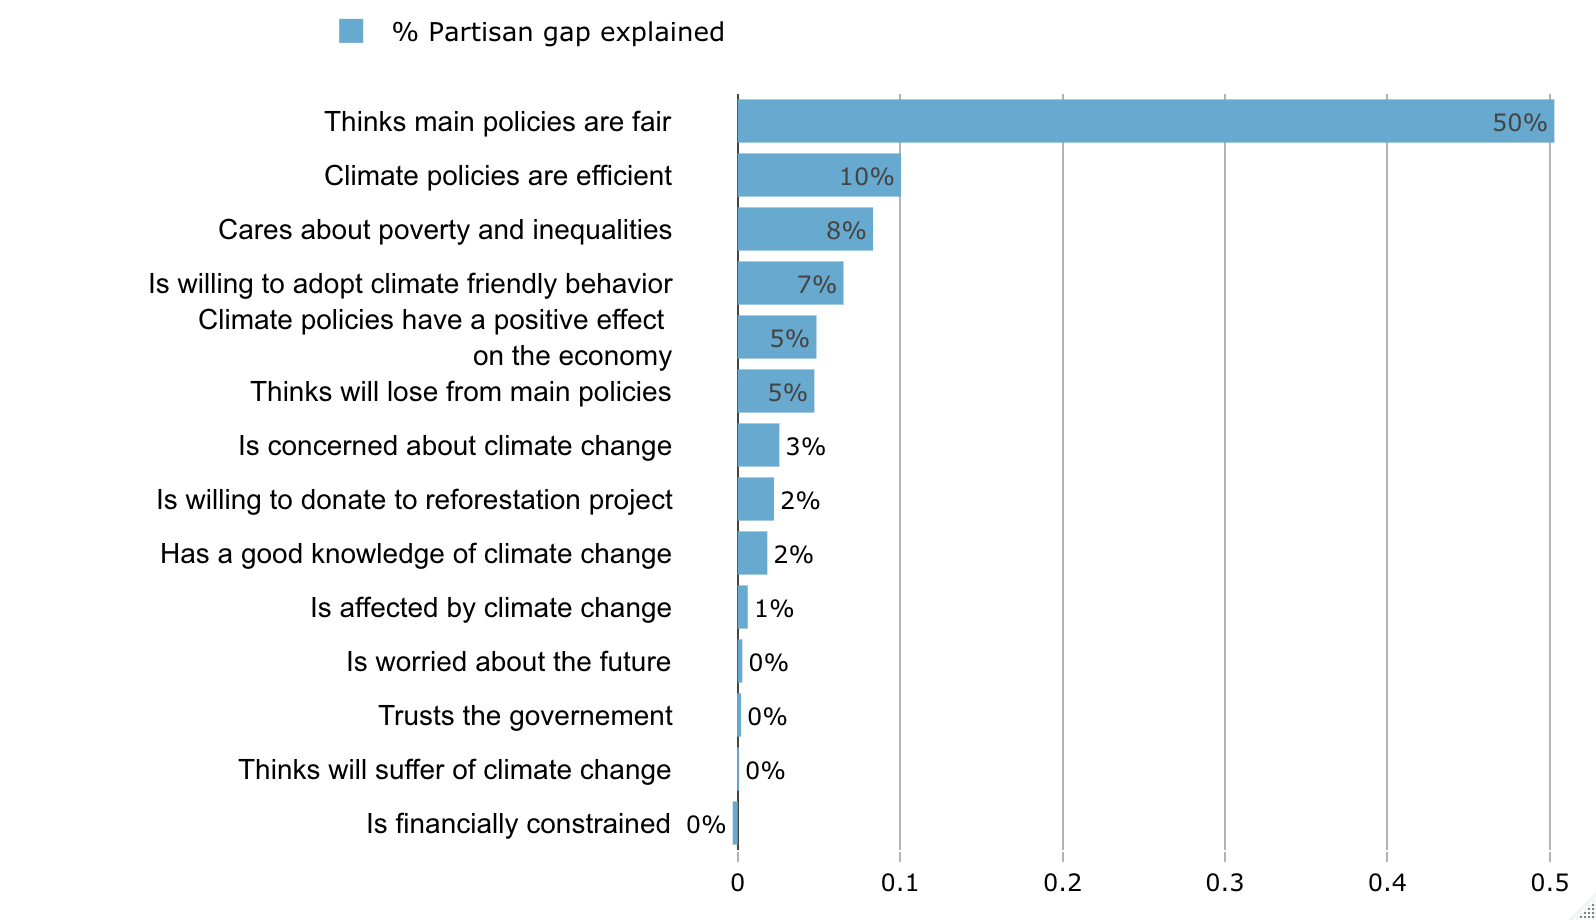
\includegraphics[width=\textwidth]{../../figures/Gelbach/gelbach_right_main_policies_D2SD}
		\end{subfigure}\\
	\end{tabular}
\end{center}
\end{figure}
\end{frame}


\begin{frame}{Gelbach decomposition of the geographical gap (urban vs. rural) in support for…}%\addtocounter{framenumber}{-1}
\vspace{-.2cm}
\begin{figure}[h!]
\caption{… all climate policies}
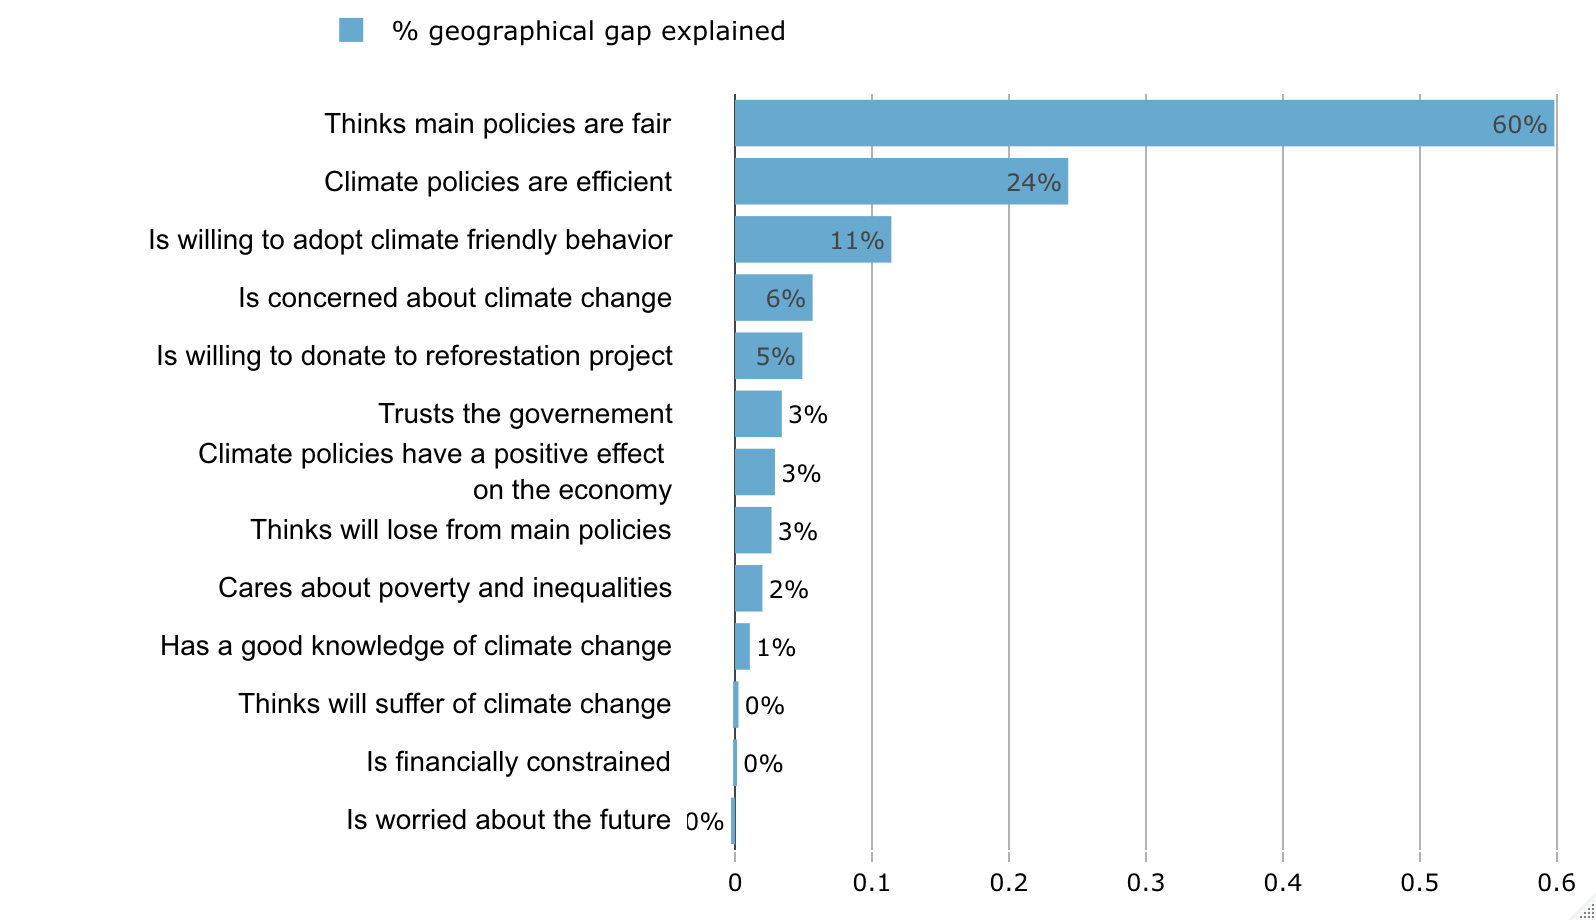
\includegraphics[width=.75\textwidth]{../../figures/Gelbach/gelbach_urban_all_policies_D2SD} \\
%\caption{Could you trust the federal goverment to implement the following policies}
{\tiny \textit{Notes:} Each bar indicates the share of the geographical gap explained by each of the factors.}
\end{figure}
\end{frame}


\begin{frame}{Explaining the Geographical Gap}
\begin{figure}[h!]
	\caption{Gelbach decomposition of the geographical gap (urban vs. rural) in support for:}
	\setlength\extrarowheight{-1pt}
\begin{center}
	\begin{tabular}{cc}
		\begin{subfigure}{0.48\textwidth}
		\caption{Ban on combustion-engine cars}
			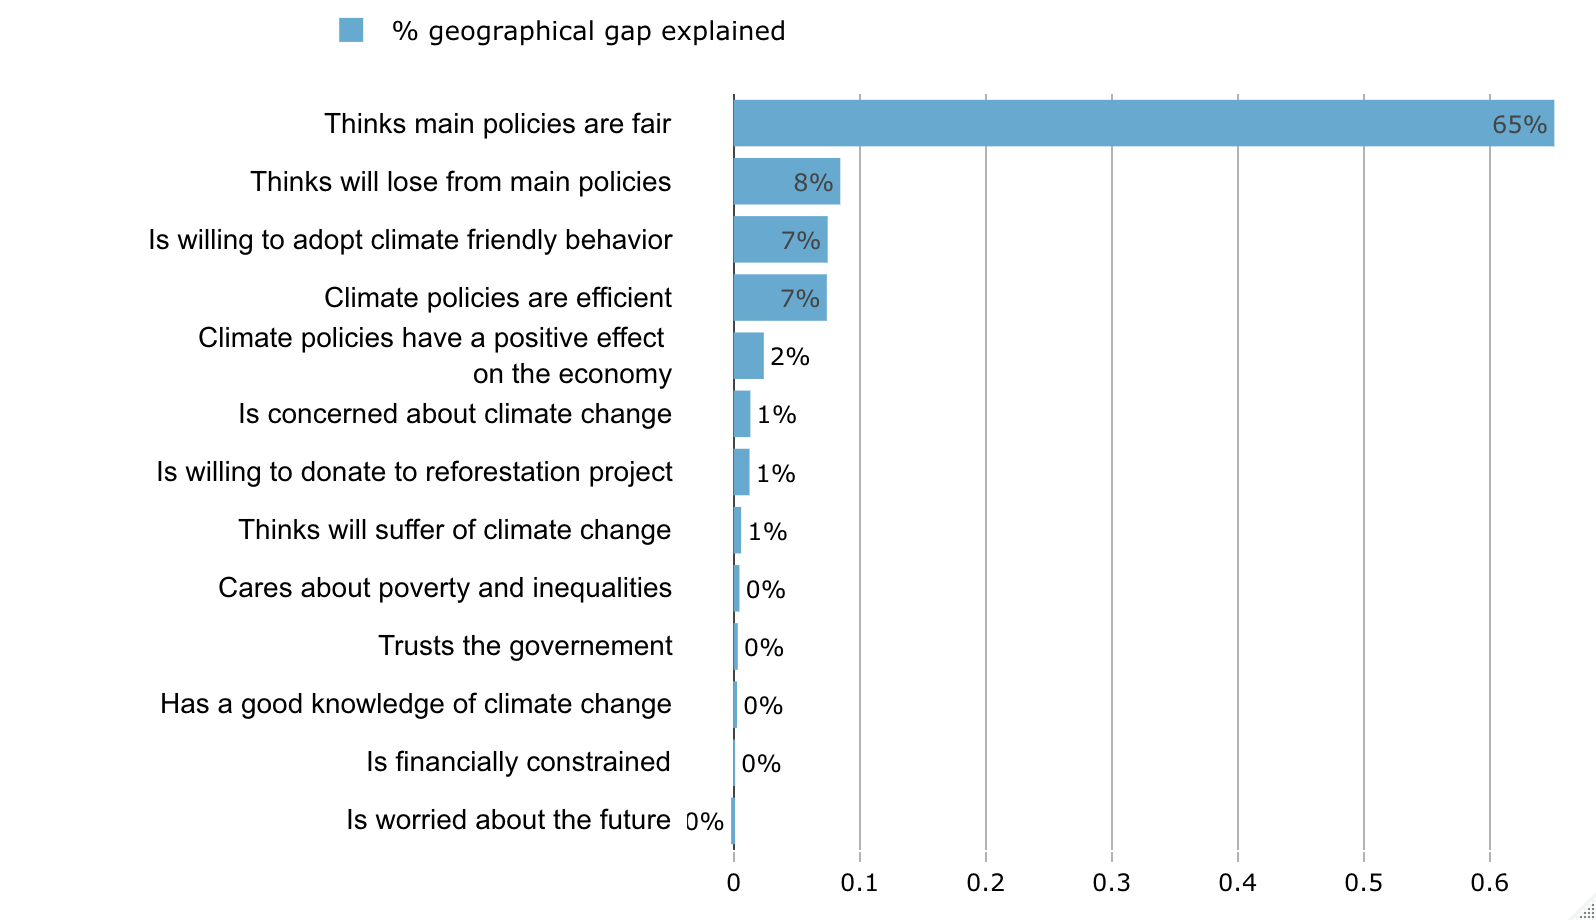
\includegraphics[width=\textwidth]{../../figures/Gelbach/gelbach_urban_standard_D2SD}
		\end{subfigure}&
		\begin{subfigure}{0.48\textwidth}
		\caption{Carbon tax with cash transfers}
			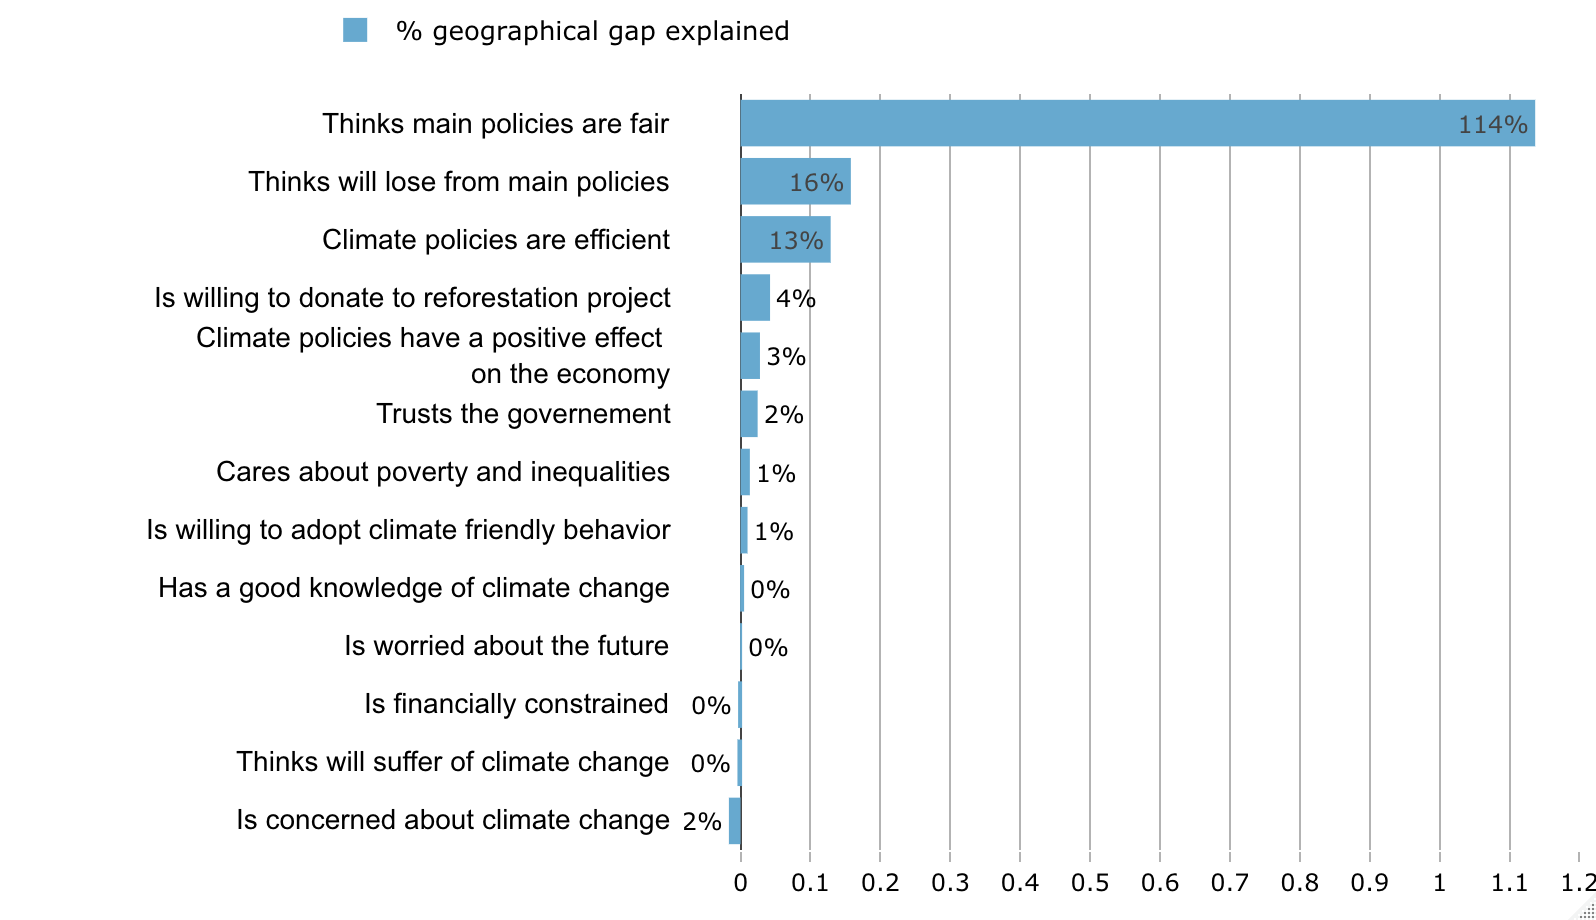
\includegraphics[width=\textwidth]{../../figures/Gelbach/gelbach_urban_tax_transfers_D2SD}
		\end{subfigure}\\
	\end{tabular}
\end{center}
\end{figure}
\end{frame}


\begin{frame}{Explaining the Geographical Gap}
\begin{figure}[h!]
	\caption{Gelbach decomposition of the geographical gap (urban vs. rural) in support for:}
	\setlength\extrarowheight{-1pt}
\begin{center}
	\begin{tabular}{cc}
		\begin{subfigure}{0.48\textwidth}
		\caption{Green investment program}
			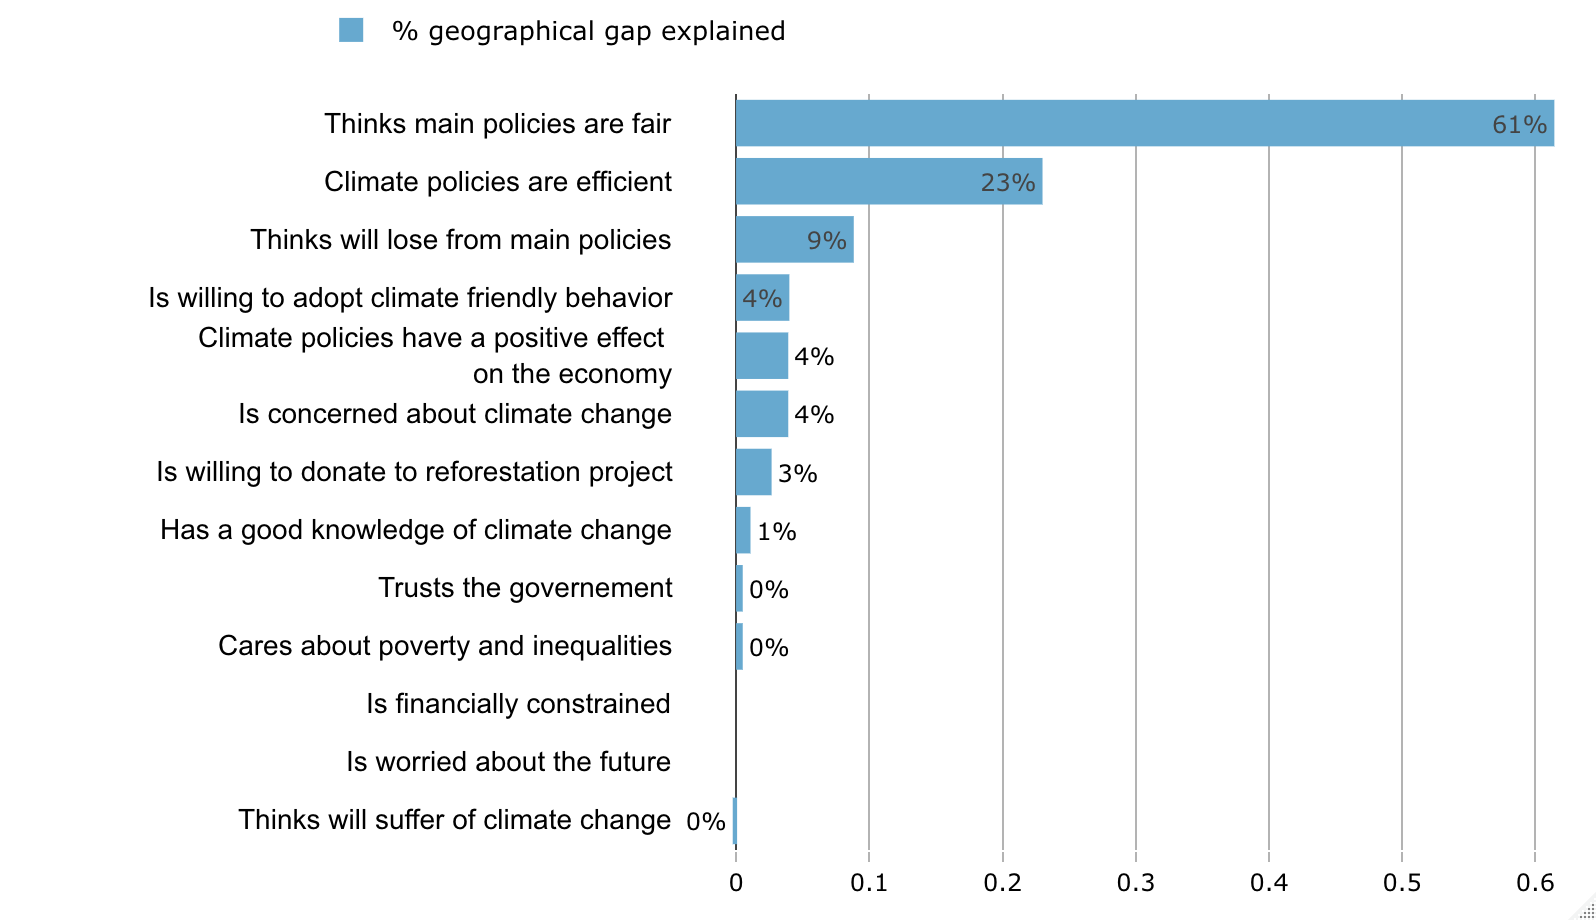
\includegraphics[width=\textwidth]{../../figures/Gelbach/gelbach_urban_investments_D2SD}
		\end{subfigure}&
		\begin{subfigure}{0.48\textwidth}
		\caption{All 3 policies}
			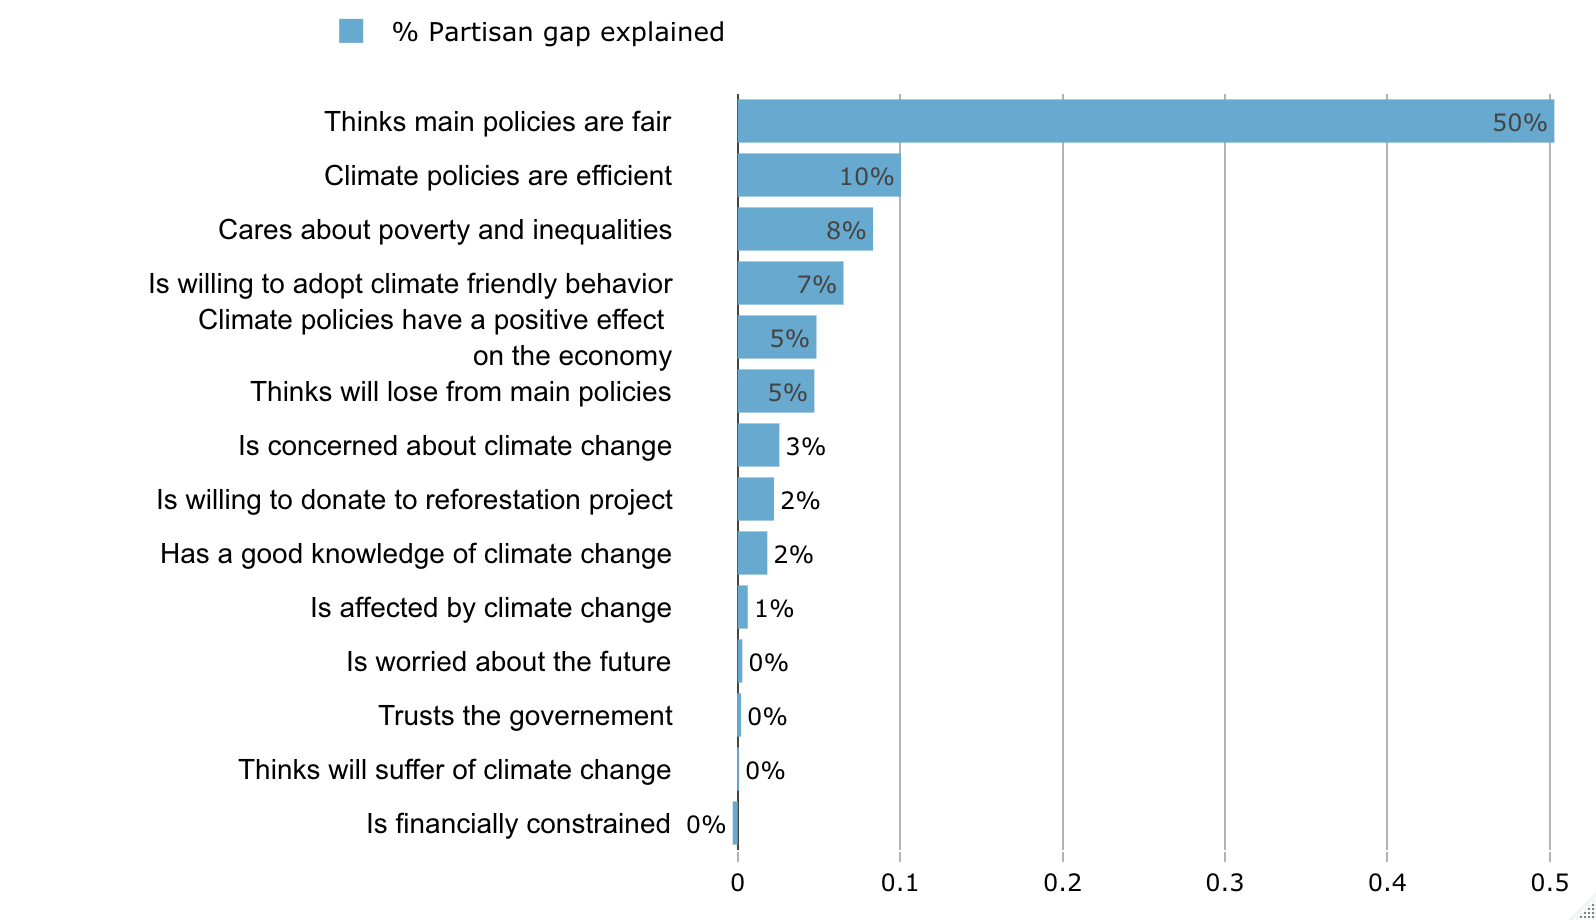
\includegraphics[width=\textwidth]{../../figures/Gelbach/gelbach_right_main_policies_D2SD}
		\end{subfigure}\\
	\end{tabular}
\end{center}
\end{figure}
\end{frame}

% \begin{frame}{Principal Component Analysis}
% % latex table generated in R 4.1.1 by xtable 1.8-4 package
% Fri Oct 22 16:05:18 2021
\begin{table}[ht]
\centering
\caption{PCA (automatic handling of missing values)}
\scalebox{.66}{
\begin{tabular}{llllllllll}
  \hline
\multicolumn{2}{c}{Component 1} & \multicolumn{2}{c}{Component 2} & \multicolumn{2}{c}{Component 3} & \multicolumn{2}{c}{Component 4} & \multicolumn{2}{c}{Component 5} \\ 
  \hline
Proportion of variance & 0.11825 &  & 0.0466 &  & 0.03628 &  & 0.02811 &  & 0.02631 \\ 
Cumulative proportion & 0.11825 &  & 0.16485 &  & 0.20113 &  & 0.22923 &  & 0.25554 \\ \hline
investments\_support & -0.136 & obstacles\_insulation\_satisfactory\_TRUE & 0.198 & employment\_agg\_Working & 0.138 & transport\_shopping\_Car\_or\_Motorbik & -0.164 & inactive\_FALSE & -0.234 \\ 
 investments\_fair & -0.134 & obstacles\_insulation\_satisfactory\_FALSE & -0.198 & country\_US & 0.136 & transport\_shopping\_Walking\_or\_Cycl & 0.154 & inactive\_TRUE & 0.234 \\ 
 should\_fight\_CC & -0.132 & home\_owner\_FALSE & -0.153 & country\_name\_United\_States & 0.136 & country\_name\_France & -0.15 & employment\_agg\_Working & -0.23 \\ 
 tax\_transfers\_support & -0.125 & home\_owner\_TRUE & 0.153 & employment\_status\_Full-time\_emplo & 0.135 & country\_FR & -0.15 & employment\_status\_Retired & 0.215 \\ 
 standard\_fair & -0.125 & watched\_policy\_Yes & 0.149 & home\_tenant\_FALSE & 0.132 & survey\_biased\_Yes,\_left & 0.145 & employment\_agg\_Retired & 0.215 \\ 
condition\_ambitious\_policies & -0.124 & know\_ban\_A\_ban\_on\_combus & 0.145 & home\_tenant\_TRUE & -0.132 & survey\_biased\_left\_FALSE & -0.145 & transport\_work\_Not\_Applicable & 0.193 \\ 
 standard\_support & -0.124 & wealth & 0.142 & home\_owner\_FALSE & -0.131 & survey\_biased\_left\_TRUE & 0.145 & transport\_work\_Car\_or\_Motorbik & -0.187 \\ 
 standard\_public\_transport\_support & -0.124 & vote\_participation\_Yes & 0.142 & home\_owner\_TRUE & 0.131 & survey\_biased\_yes\_TRUE & 0.143 & affected\_transport & -0.175 \\ 
tax\_transfers\_fair & -0.123 & voted\_FALSE & -0.142 & standard\_win\_lose\_poor & 0.129 & survey\_biased\_yes\_FALSE & -0.143 & employment\_status\_Full-time\_emplo & -0.174 \\ 
CC\_problem & -0.123 & voted\_TRUE & 0.142 & inactive\_FALSE & 0.127 & survey\_biased\_No & -0.143 & age\_65+ & 0.173 \\ 
   \hline
\end{tabular}
}
\end{table}

% \end{frame}

\begin{frame}{Principal Component Analysis (PCA)}
\input{../../tables/PCA/pca_all_missing_mean.tex}
\end{frame}

\begin{frame}{Decision tree}
	\begin{figure}
		\caption{Decision tree for the Support to the 3 main policies}
		\includegraphics[height=.85\textheight]{../../figures/all/tree_main_policies.png}		
	\end{figure}
\end{frame}
	

\end{document}